% Copyright 2004 by Till Tantau <tantau@users.sourceforge.net>.
%
% In principle, this file can be redistributed and/or modified under
% the terms of the GNU Public License, version 2.
%
% However, this file is supposed to be a template to be modified
% for your own needs. For this reason, if you use this file as a
% template and not specifically distribute it as part of a another
% package/program, I grant the extra permission to freely copy and
% modify this file as you see fit and even to delete this copyright
% notice. 

\documentclass{beamer}

% There are many different themes available for Beamer. A comprehensive
% list with examples is given here:
% http://deic.uab.es/~iblanes/beamer_gallery/index_by_theme.html
% You can uncomment the themes below if you would like to use a different
% one:
%\usetheme{AnnArbor}
%\usetheme{Antibes}
%\usetheme{Bergen}
%\usetheme{Berkeley}
%\usetheme{Berlin}
%\usetheme{Boadilla}
%\usetheme{boxes}
%\usetheme{CambridgeUS}
%\usetheme{Copenhagen}
%\usetheme{Darmstadt}
\usetheme{default}
%\usetheme{Frankfurt}
%\usetheme{Goettingen}
%\usetheme{Hannover}
%\usetheme{Ilmenau}
%\usetheme{JuanLesPins}
%\usetheme{Luebeck}
%\usetheme{Madrid}
%\usetheme{Malmoe}
%\usetheme{Marburg}
%\usetheme{Montpellier}
%\usetheme{PaloAlto}
%\usetheme{Pittsburgh}
%\usetheme{Rochester}
%\usetheme{Singapore}
%\usetheme{Szeged}
%\usetheme{Warsaw}

\usepackage{setspace} 
\usepackage{amsmath}
\usepackage{graphicx}
\newcommand*{\LargerCdot}{\raisebox{-0.25ex}{\scalebox{2.3}{$\cdot$}}}

\usepackage{color}
%\input{rgb}

\definecolor{red1}{rgb}{1.000000,0.000000,0.000000}

\title{Quote-rate trending analysis}

% A subtitle is optional and this may be deleted
%\subtitle{A study of Turbulence in Financial Markets}

\author{Ranaji~Krishna}
% - Give the names in the same order as the appear in the paper.
% - Use the \inst{?} command only if the authors have different
%   affiliation.

%\institute[Universities of Somewhere and Elsewhere] % (optional, but mostly needed)
%{
%  \inst{1}%
%  Summer Intern\\
%  Research Affiliates
%  \and
%  \inst{2}%
%  Vice President Research\\
%  Research Affiliates}
% - Use the \inst command only if there are several affiliations.
% - Keep it simple, no one is interested in your street address.

%\date{2013}
% - Either use conference name or its abbreviation.
% - Not really informative to the audience, more for people (including
%   yourself) who are reading the slides online

\subject{Theoretical Computer Science}
% This is only inserted into the PDF information catalog. Can be left
% out. 

% If you have a file called "university-logo-filename.xxx", where xxx
% is a graphic format that can be processed by latex or pdflatex,
% resp., then you can add a logo as follows:

\pgfdeclareimage[height=0.6cm]{university-logo}{thm_logo.png}
\logo{\pgfuseimage{university-logo}}

% Delete this, if you do not want the table of contents to pop up at
% the beginning of each subsection:
%\AtBeginSubsection[]
%{
%  \begin{frame}<beamer>{Outline}
%    \tableofcontents[currentsection,currentsubsection]
%  \end{frame}
%}^6

% Let's get started
\begin{document}

\begin{frame}
  \titlepage
\end{frame}

%\begin{frame}{Outline}
%%	\begin{scriptsize}
%	 		\tableofcontents
%%  		% You might wish to add the option [pausesections]
%%	\end{scriptsize}
%\end{frame}

% Section and subsections will appear in the presentation overview
% and table of contents.
%\section{\small{Turbulence}}
	%\section{\small{The Concept of Financial Turbulence}}
	%\section{Turbulence as a measure of Systemic risk}
	% What are the other forms of systemic risk

%\setlength\listparindent{1in}

\begin{frame}{Problem Statement}{}
	\begin{itemize}
		\item{To identify whether service providers are becoming more or less inclined to quote over time?}\vspace{0.5 in}
		\item{To explore if there is evidence that product changes over the last two months have caused site-wide shifts in quoting behavior?} \vspace{0.5 in}
	\end{itemize}
\end{frame}

\begin{frame}{Approach}{}
	\begin{itemize}
			
		\item{It was envisaged that site-wide shifts would affect the quoting behavior across all service providers. Therefore quote-rates for invited service providers were computed every hour, and an equally weighted average of the ratios was computed for the hour.} \vspace{0.5in}	
		
		\item{An estimation model of quote-rate (dependent variable) against time (independent variable) was developed; the significance of time in estimating quote-rate was investigated.} \vspace{0.5 in}
		
	%	\item{It was envisaged that site-wide shifts would affect the quoting behavior across all service providers. Therefore ratios reflecting quote-rate had to be constructed such that they would be able to distinguish changes across service providers from those due to individual service providers.}
	\end{itemize}
\end{frame}

\begin{frame}{Data Cleaning}{}
	\begin{itemize}
		\item{A table containing entries of ``requests sent", ``invites sent", ``quotes received", ``locations", ``categories" and ``users"  was created from relational databases containing historical data using SQLite.}\vspace{0.1 in}
		\item{An average quote-invite ratio was computed for every hour. This was done as follows:} \newline
		{$\LargerCdot$ for each invited service provider in an hour, a quote-invite ratio was computed by diving the number of invites that led to quotes by the total number of invites received;}\newline 
		{$\LargerCdot$ then an average quote-invite ratio was computed across the service providers for the hour.}\newline
		\item{ This yielded  {\color{blue}1502} quote-invite ratios from the historical data set which contained dates of ``invites sent" spanning from {\color{blue}{1 July 2013 - 2 September 2013}}.}
%		\item{Computing ratios for each service provider and averaging across all service providers would capture systemic changes whilst being robust to idiosyncrasies of service providers.}
		\end{itemize}
\end{frame}

\begin{frame}{Estimation technique}{}
	\begin{itemize}		
		%\item{This would distinguish changes in qr due to systemic changes from idio changes of sp. }\vspace{0.1 in}
		\vspace{-0.1in}
		\item{Trends of quote-invite ratio are shown below:}\vspace{0.1 in}
	\begin{figure}
		\begin{itemize}
			\begin{center}
				\vspace*{-0.1in}
				\hspace*{-0.8in}
				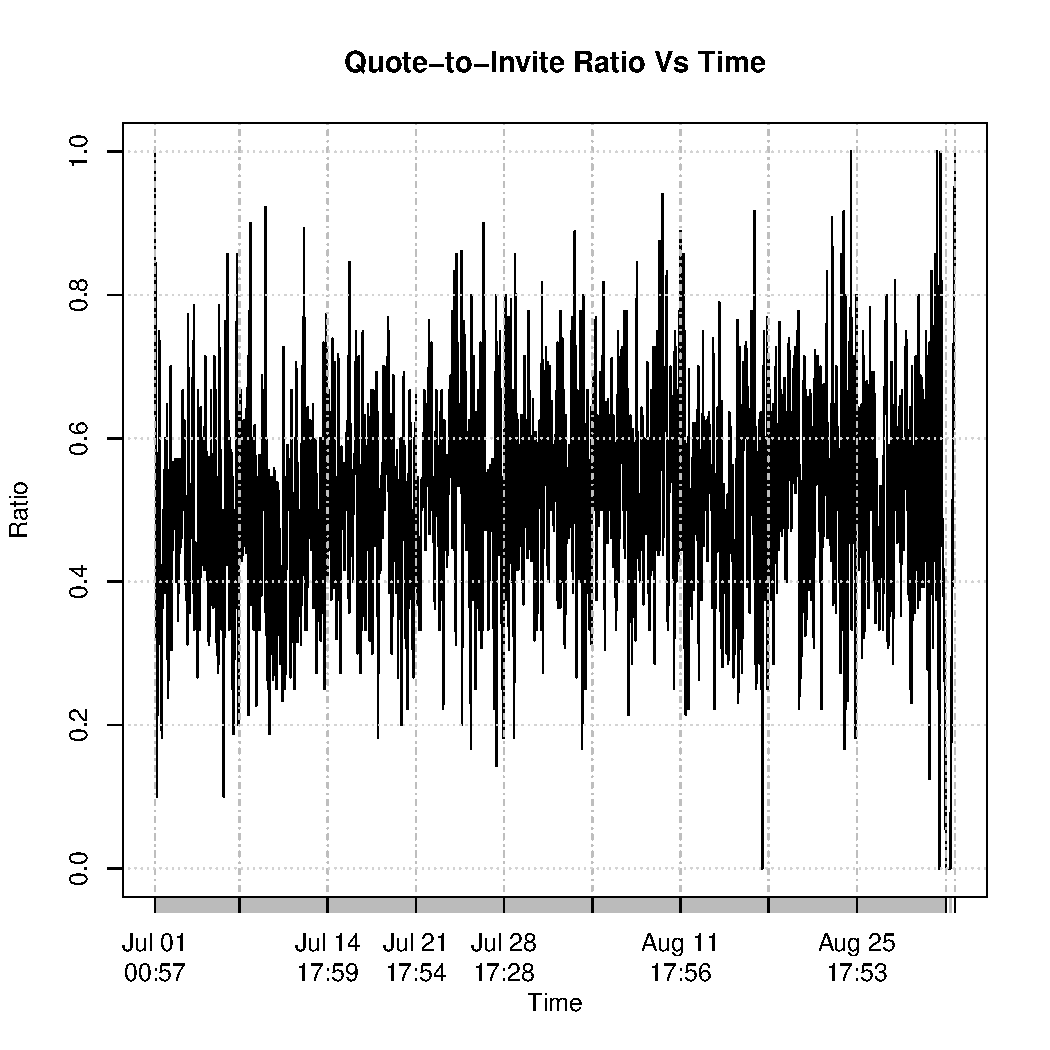
\includegraphics[width=0.55\textwidth]{hr_plot.pdf} 
	 			 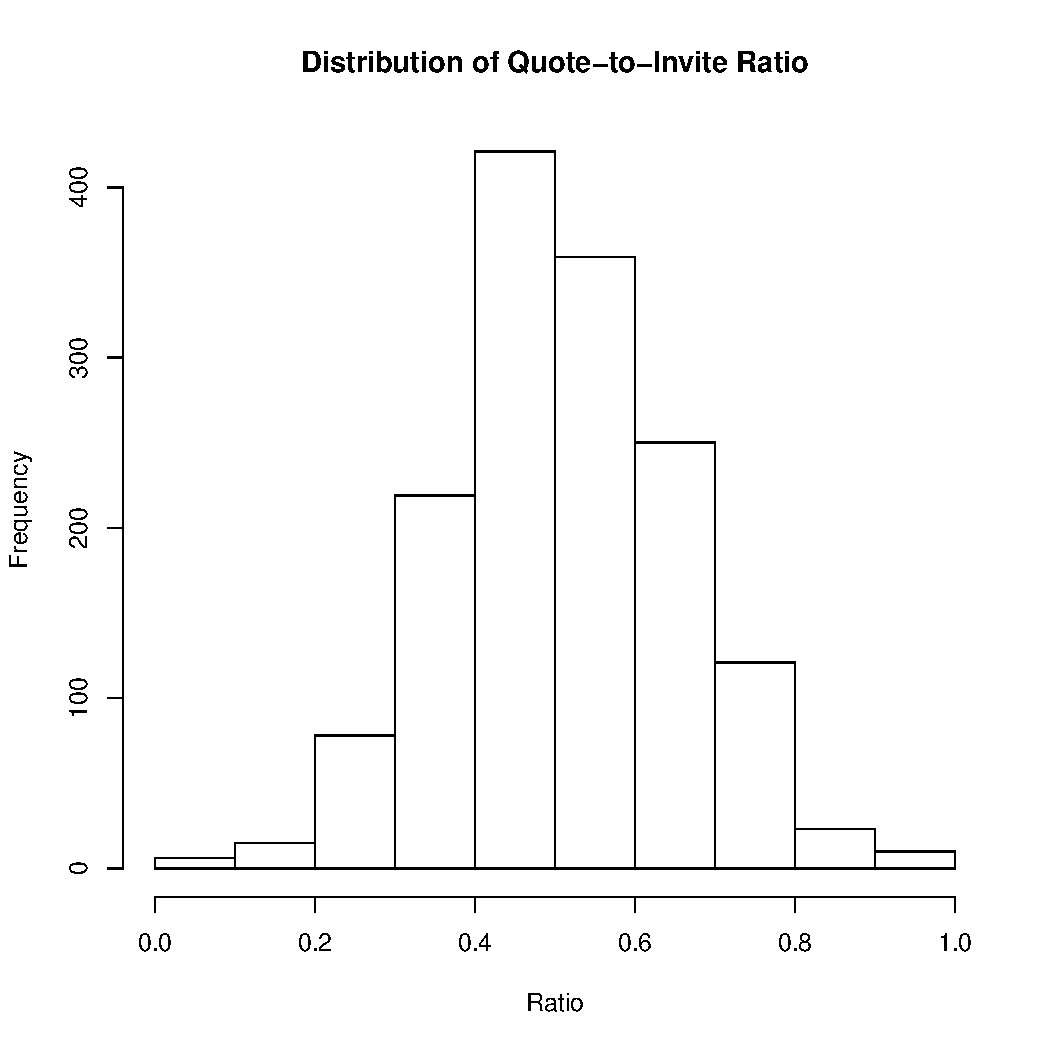
\includegraphics[width=0.55\textwidth]{hr_dist.pdf} 
			\end{center}
		\end{itemize}
	\end{figure}
%	\begin{figure}{}
%		\vspace*{-0.1 in}
%		\scalebox{0.5}
%		{\hspace*{-0.3 in}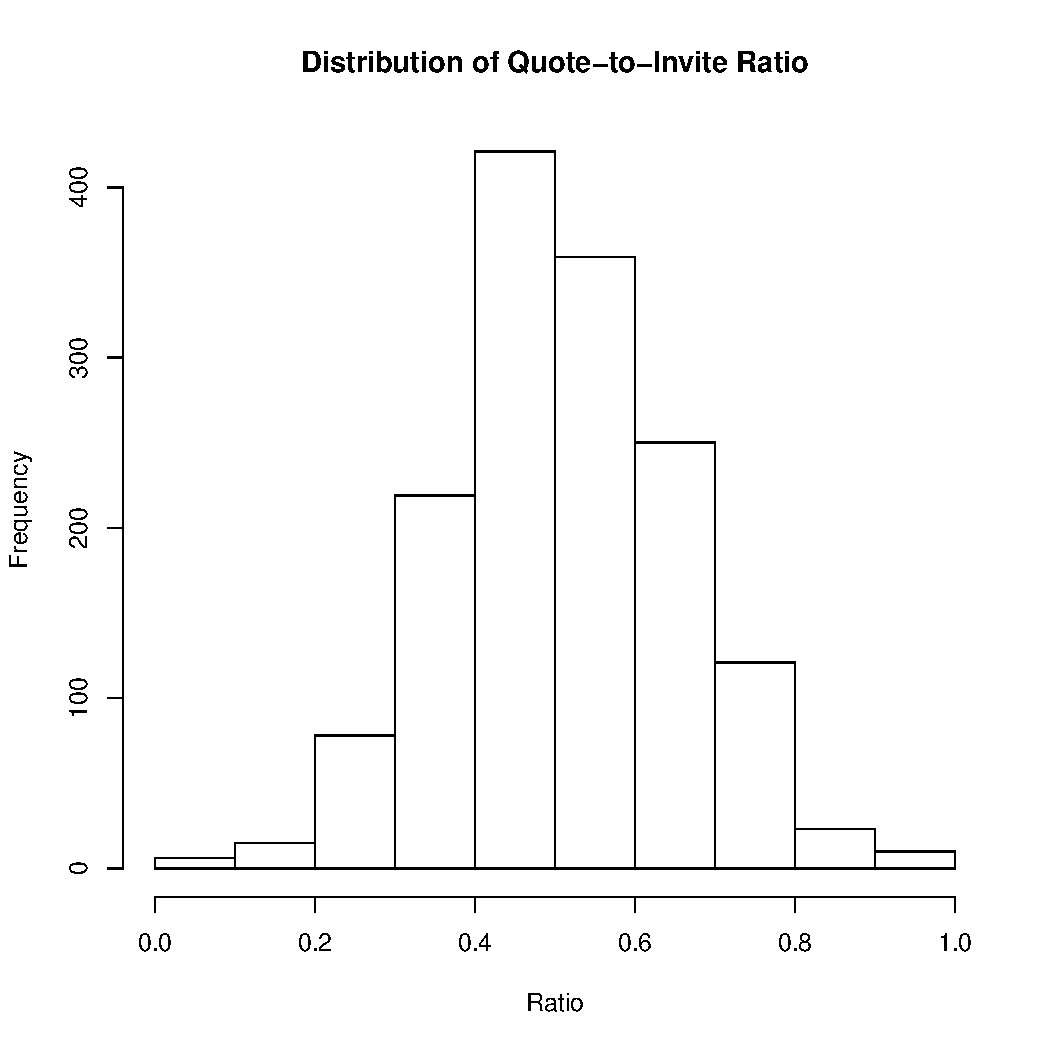
\includegraphics[scale=0.7]{hr_dist.pdf} }
%	\end{figure}
		%\item{Since the values are range between $0$ and $1$ use a {\color{blue}{zero-and-one inflated beta distribution model}} .}
		\end{itemize}
\end{frame}

\begin{frame}{Estimation technique}{contd.}
	\begin{itemize}
		%\item{We note that the values range between $0$ and $1$. The usual practice is to transform the data using logit, $\tilde{y} = log(y/1-y)$.}\newline
		\item{Regression models involving data from the unit interval, such as proportions, are typically modeled using beta distributions.}\newline
		\item{However, beta distribution for the response variable cannot be used due to inclusion of zeros and ones.}\newline
		\item{A logit transformation works if we make all zeros slightly more than zero and all ones slightly less than one.  However, this introduces a certain amount of arbitrary bias into the model.}\newline
		
		\item{We use a {\color{blue}{zero-and-one inflated beta distribution model}} (mixture of a Beta and a Bernoulli distribution) for our purpose.}
		\end{itemize}
\end{frame}
		
\begin{frame}{Results}{}
	\vspace{-0.1 in}
	\begin{figure}{}
		\vspace*{-0 in}
		\scalebox{1}
		{\hspace*{-0 in}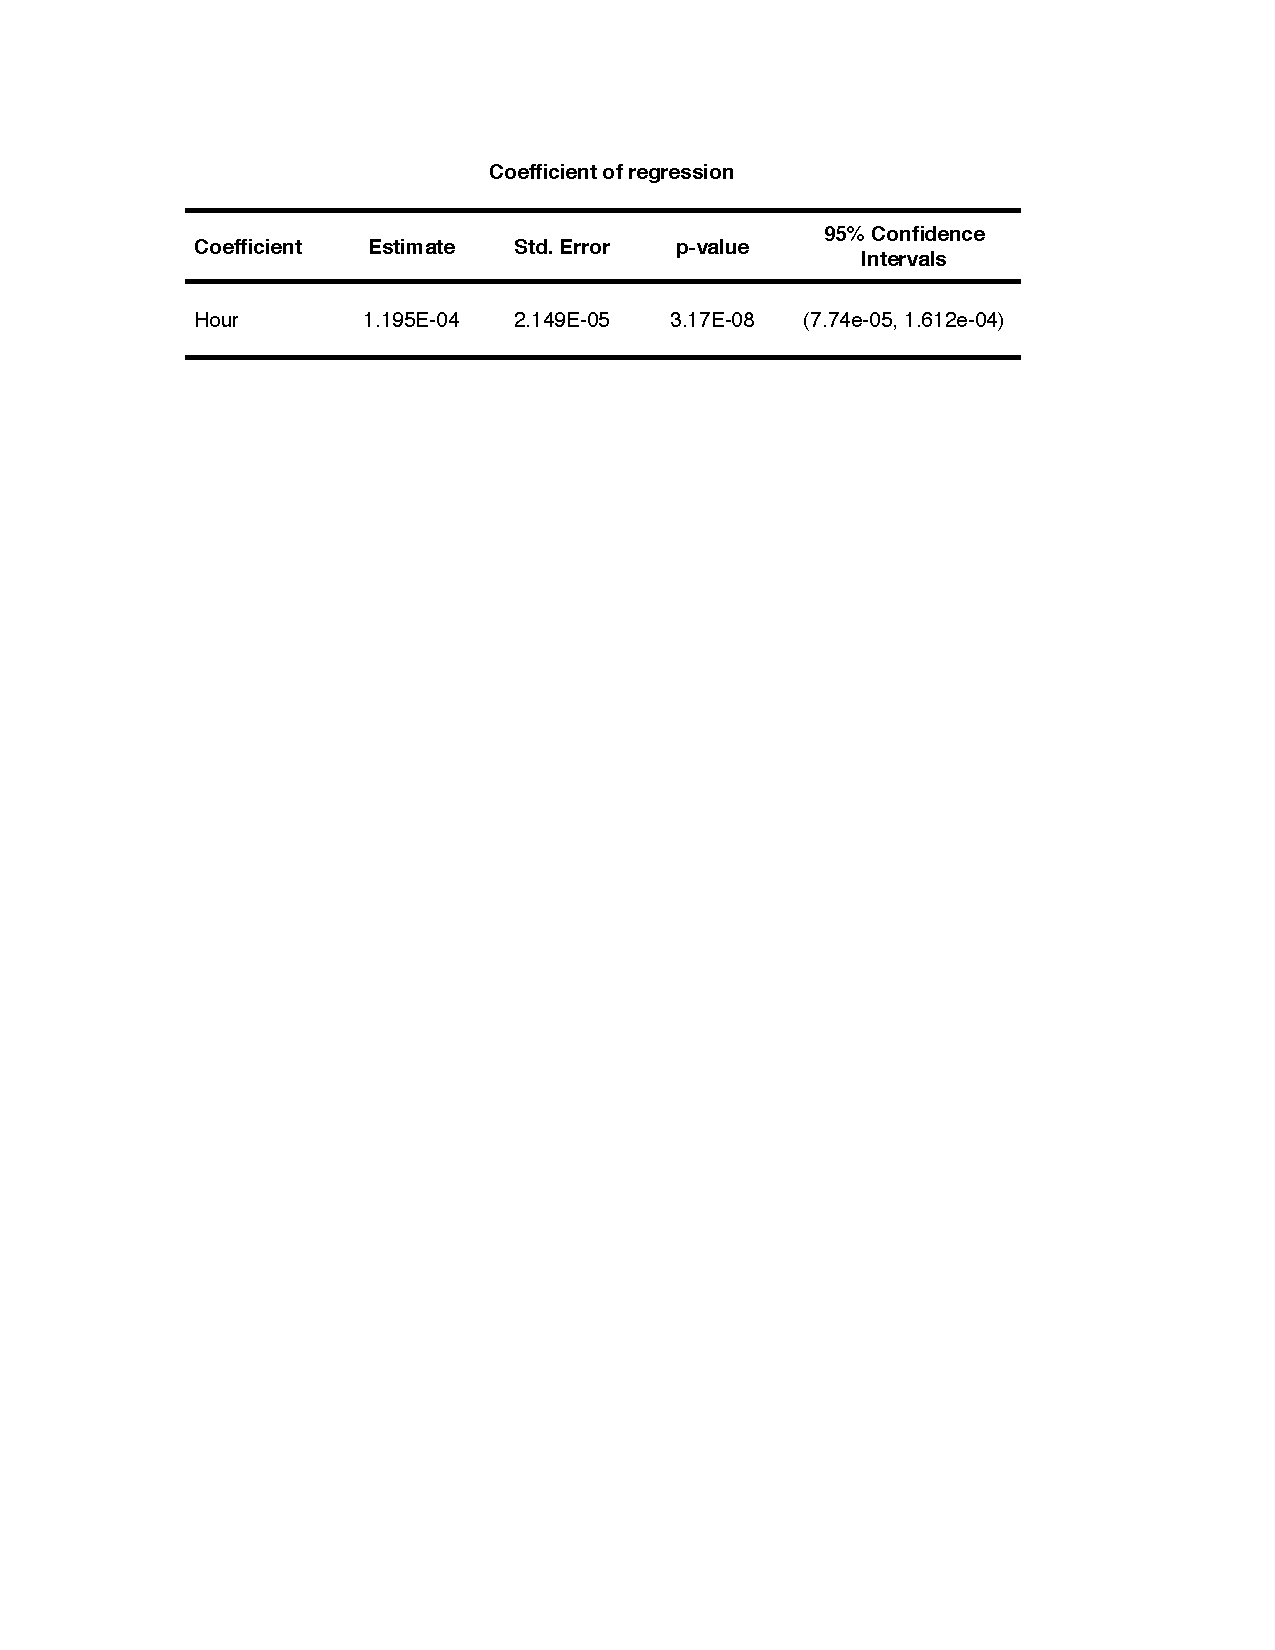
\includegraphics[scale=0.7]{coefficient.pdf} }
	\end{figure}	
	\vspace*{-0 in}
	
	\begin{figure}
		\begin{itemize}
			\begin{center}
				\vspace*{-0.5in}
				\hspace*{-0.3in}
				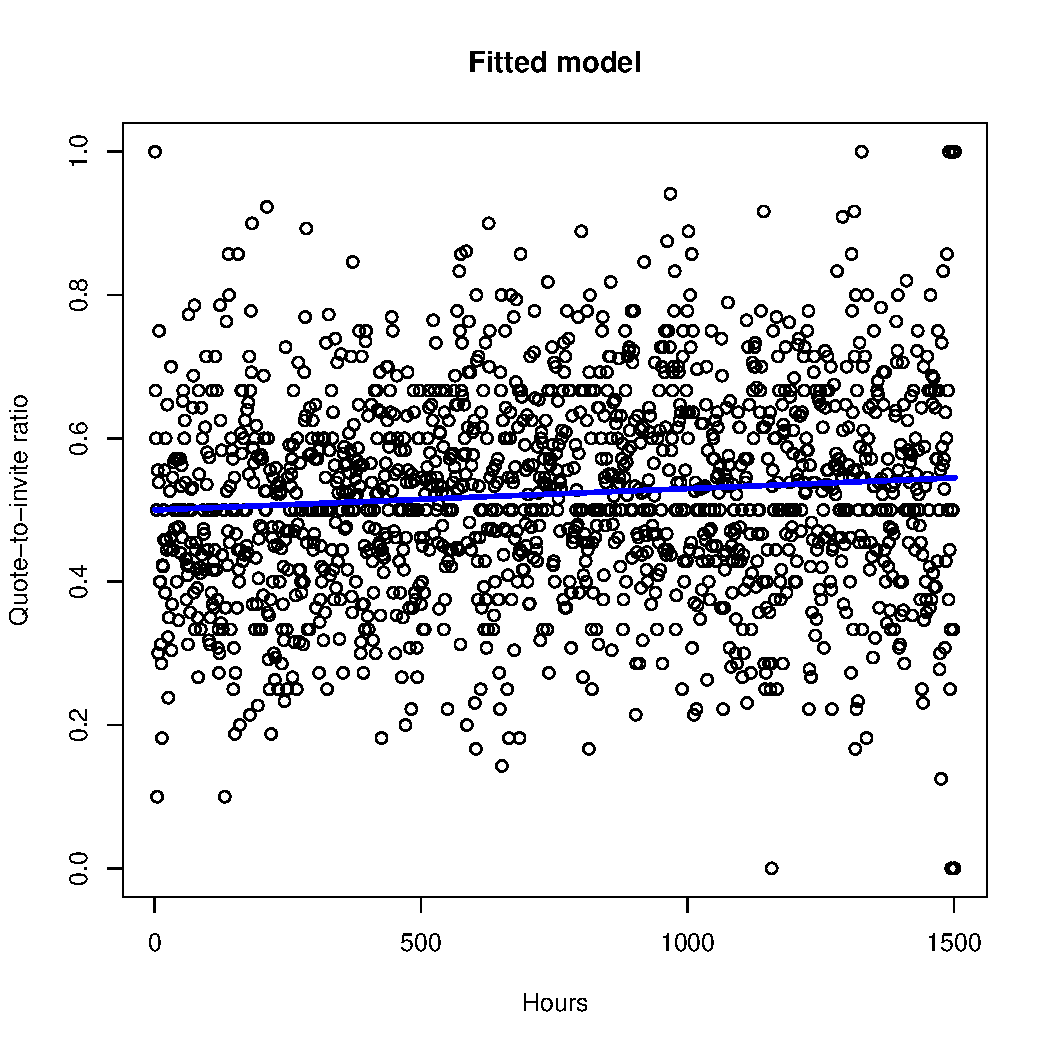
\includegraphics[width=0.5\textwidth]{scat_fit.pdf} 
	 			 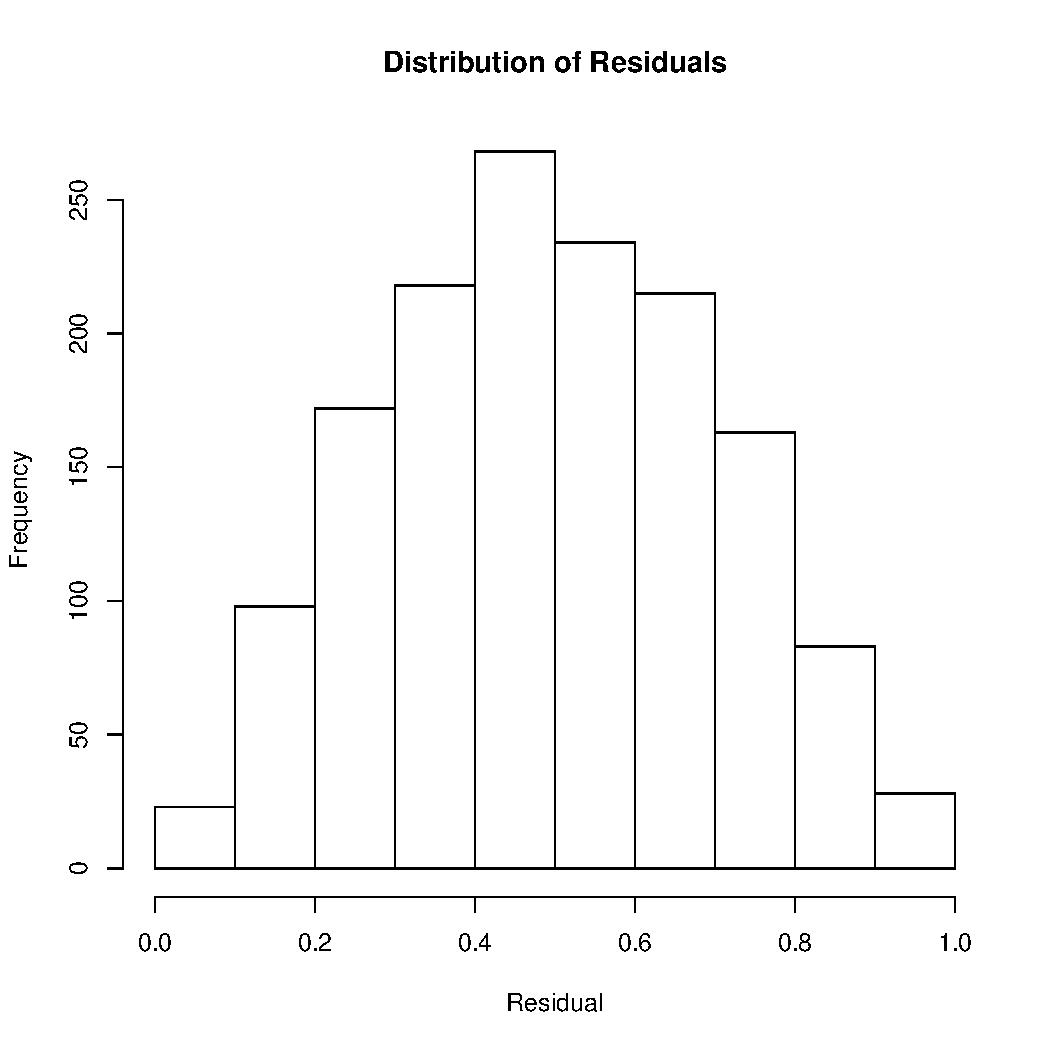
\includegraphics[width=0.5\textwidth]{res_dist.pdf} 
			\end{center}
		\end{itemize}
	\end{figure}
	\begin{itemize}
		\vspace{-0.25in}
		\item {Computations for fitting the model were carried out using the package \textbf{gamlss} in R.} 
	\end{itemize}
\end{frame}

\begin{frame}{Interpretation of Coefficient}{}
\vspace{-0in}
	\begin{itemize}
		\item {We note that the ``Hour" has significant explanatory power in estimating quote-invite ratio.}\newline\vspace{-0in}		
		\item{The model can be expressed as:}\newline
	\begin{equation}
		\ln\Big(\frac{q/i}{1-q/i}\Big) = 1.195e^{-04} \times hr
	\end{equation} where $q/i$ is the quote-to-invite ratio and $hr$ is the hour variable.\newline
		\item{The coefficient can be interpreted as the percentage change in ``quote-invite" to ``no quote-invite" ratio, due to $1\%$ increase in hour.}\newline
		\end{itemize}
\end{frame}		
%		
\begin{frame}{Interpretation of Coefficient}{contd.}
\vspace{-0.15in}
	\begin{itemize}
		\item{A positive coefficient shows improvement in the invite-quote ratio; it reveals that service providers are becoming more inclined to quote over time.}\newline
	
		\item{Example:\newline
		An hour has an average of $9$ quotes sent for $10$ invites received across invited service providers, generating a ``quote-invite" to ``no quote-invite" ratio of $9$. After $100$ days the ratio is expected to increase by $28.68\%$ to $11.58$. Therefore after $100$ days, for $10$ invites sent, $9.21$ quotes are expected to be received.}\newline
		
	\end{itemize}
\end{frame}		
		
\begin{frame}{Behavior across Categories}{}
	\vspace{0 in}
	\begin{itemize}
		\item {The analysis was performed for each {\color{blue}{Category}}.}\newline
		\item{Categories that had coefficients with significant explanatory power were analyzed.}\newline
		\item {Categories with positive coefficients:}\newline 
	\end{itemize}
		\vspace{-0.3 in}
	\begin{figure}{}
		\vspace*{-0 in}
		\scalebox{1}
		{\hspace*{-0 in}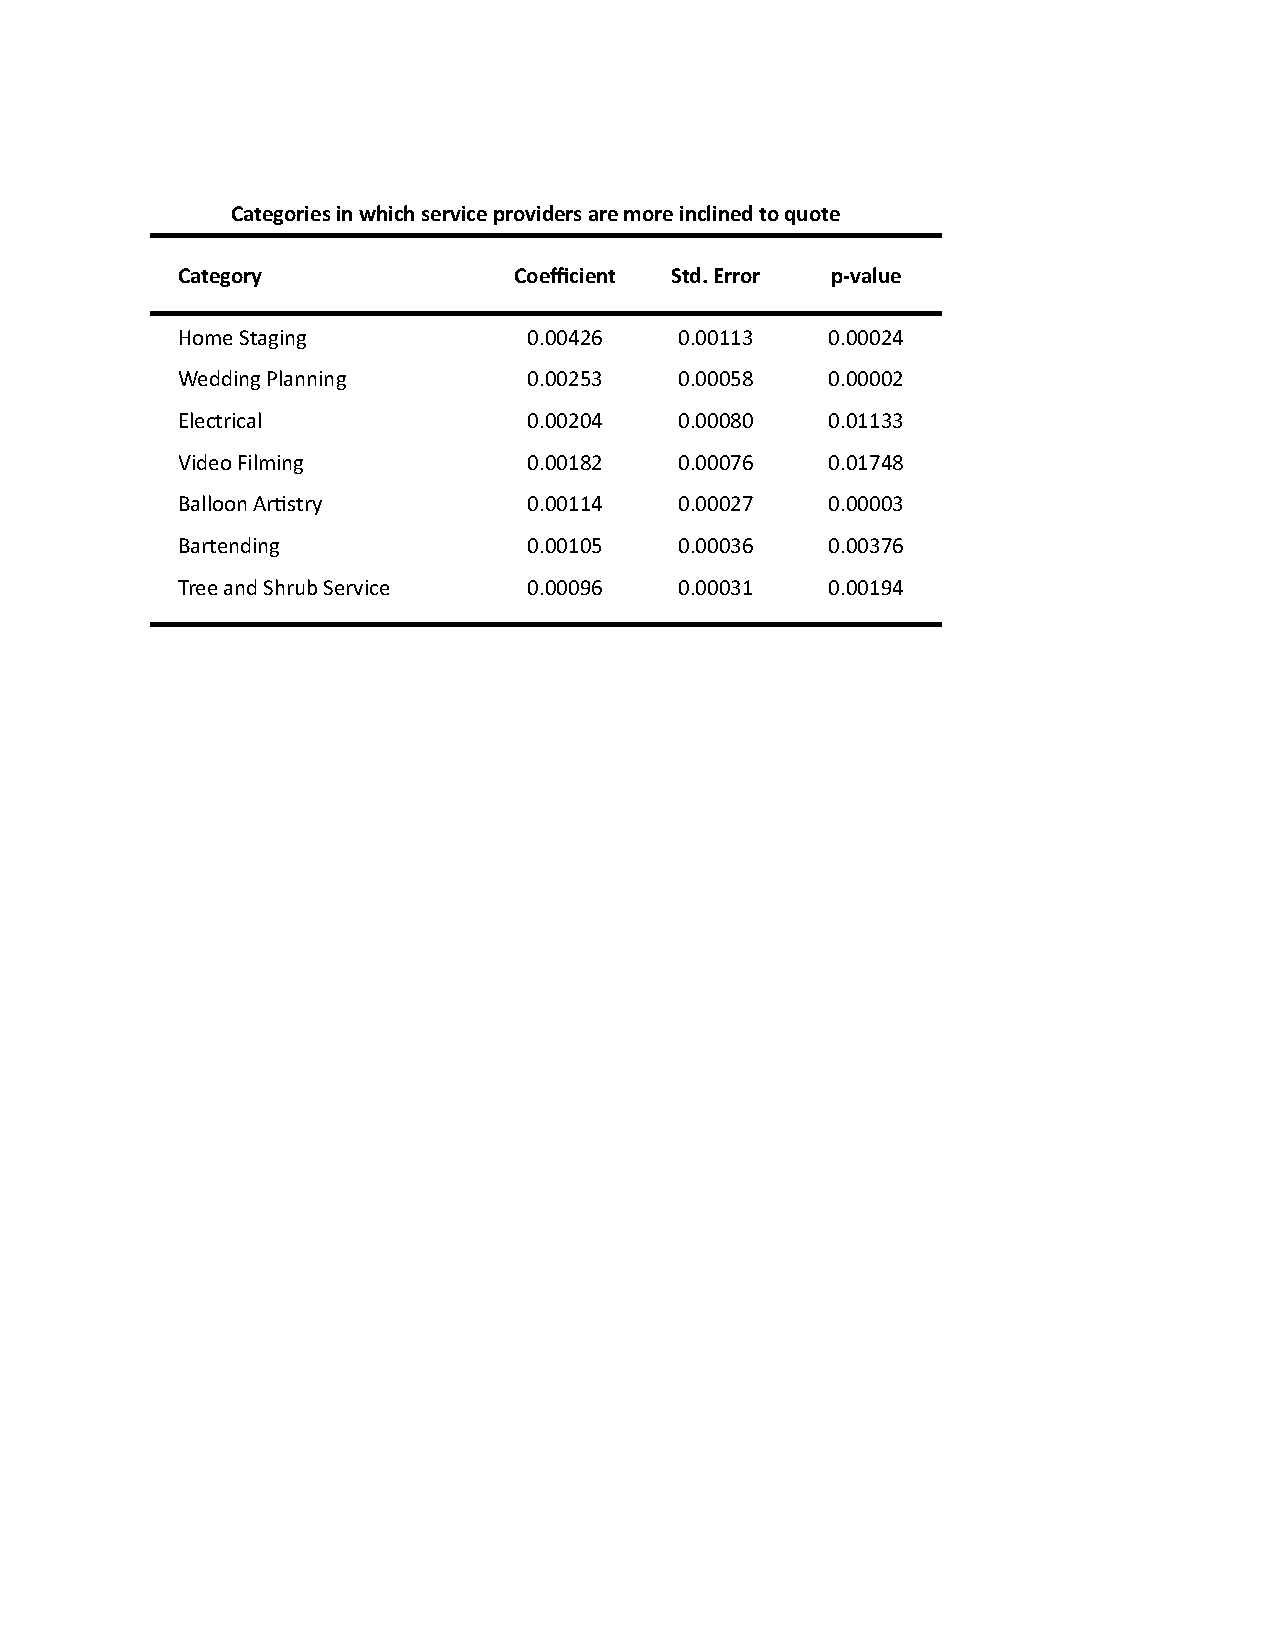
\includegraphics[scale=0.7]{coef_cat_more.pdf} }
	\end{figure}	
	\vspace*{-0 in}
\end{frame}
		
\begin{frame}{Behavior across Categories}{contd.}
	\vspace{-0. in}
	\begin{itemize}
		\item {Categories with negative coefficients:}  
	\end{itemize}
		\vspace{-0.1 in}
	\begin{figure}{}
		\vspace*{-0 in}
		\scalebox{1}
		{\hspace*{-0 in}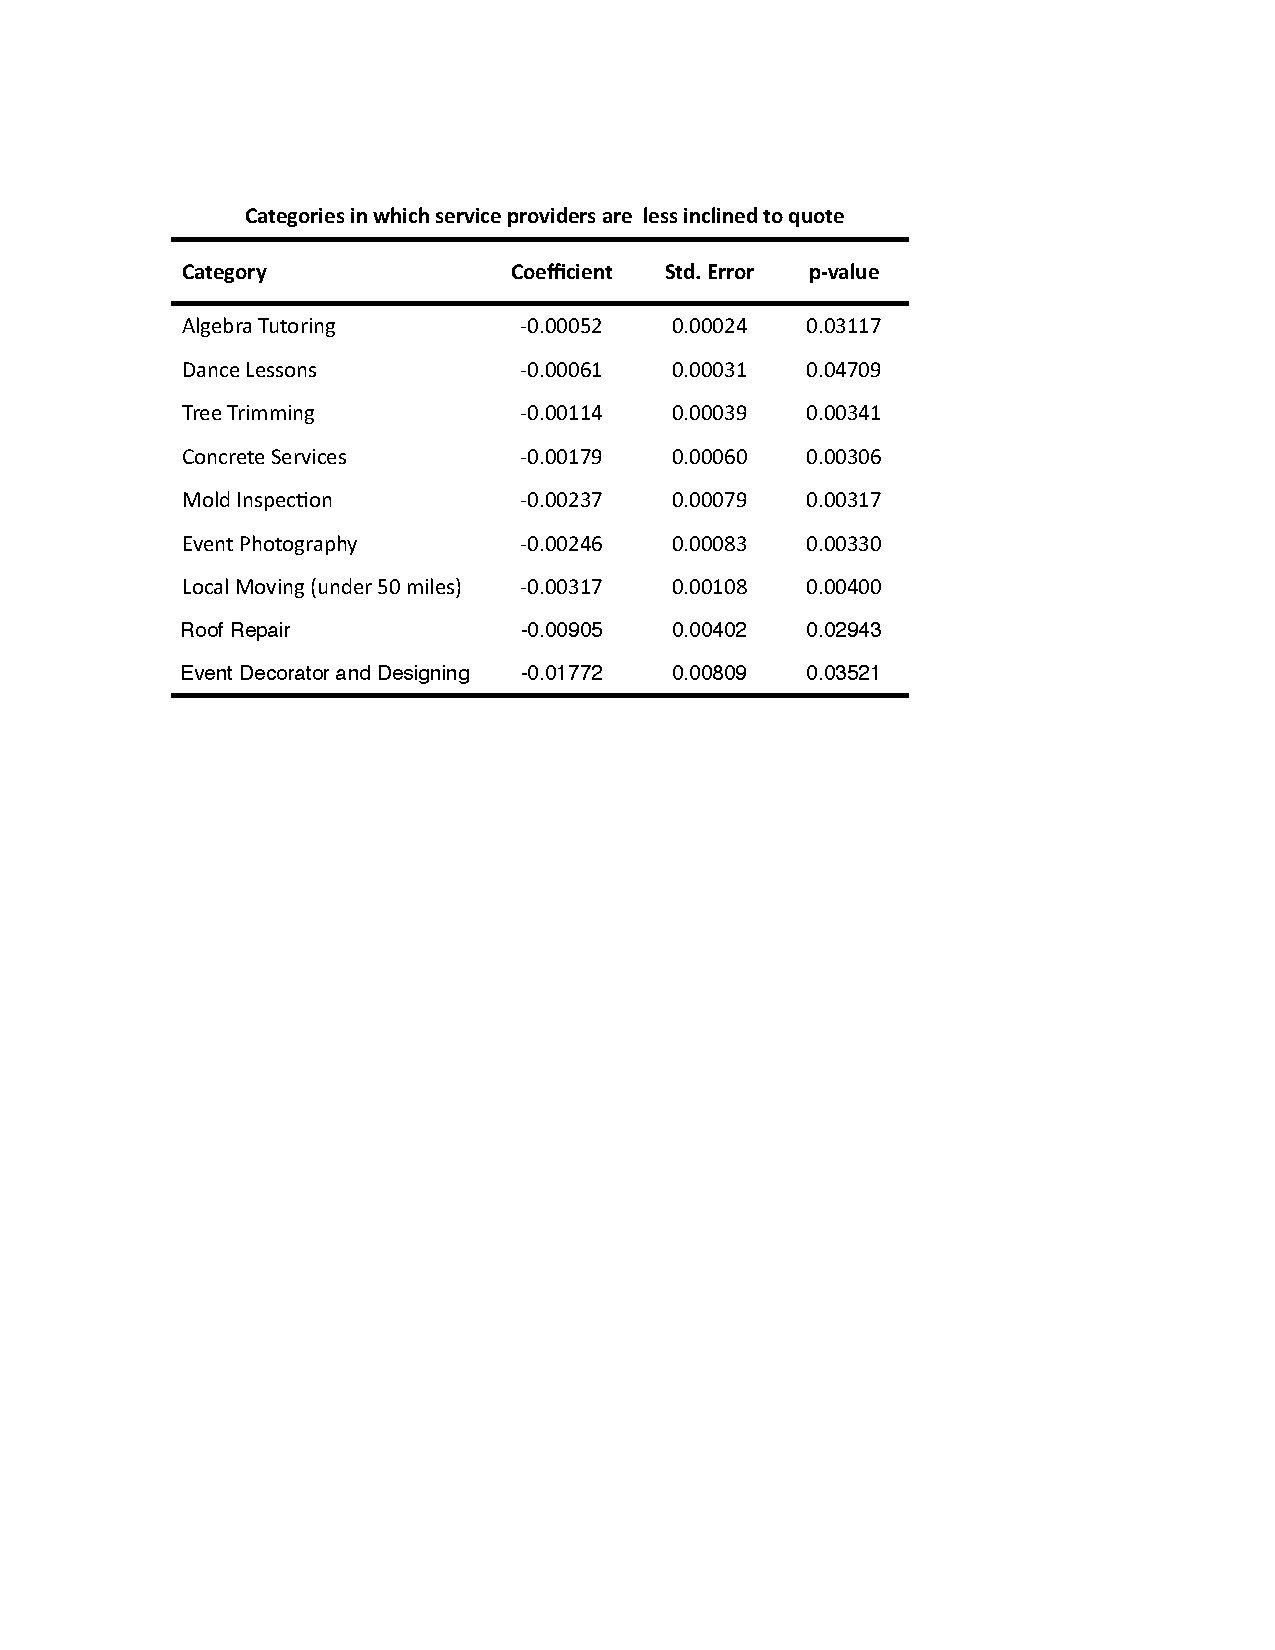
\includegraphics[scale=0.7]{coef_cat_less.pdf} }
	\end{figure}	
	\vspace*{-0 in}
\end{frame}		

\begin{frame}{Behavior across Locations}{}
	\vspace{-0. in}
	\begin{itemize}
		\item {The analysis was performed for each {\color{blue}{Location}}.}\newline
		\item{Locations that had coefficients with significant explanatory power were analyzed.}\newline
		\item {Locations with positive coefficients:}\newline 
	\end{itemize}
		\vspace{-0.6 in}
	\begin{figure}{}
		\vspace*{-0 in}
		\scalebox{1}
		{\hspace*{-0 in}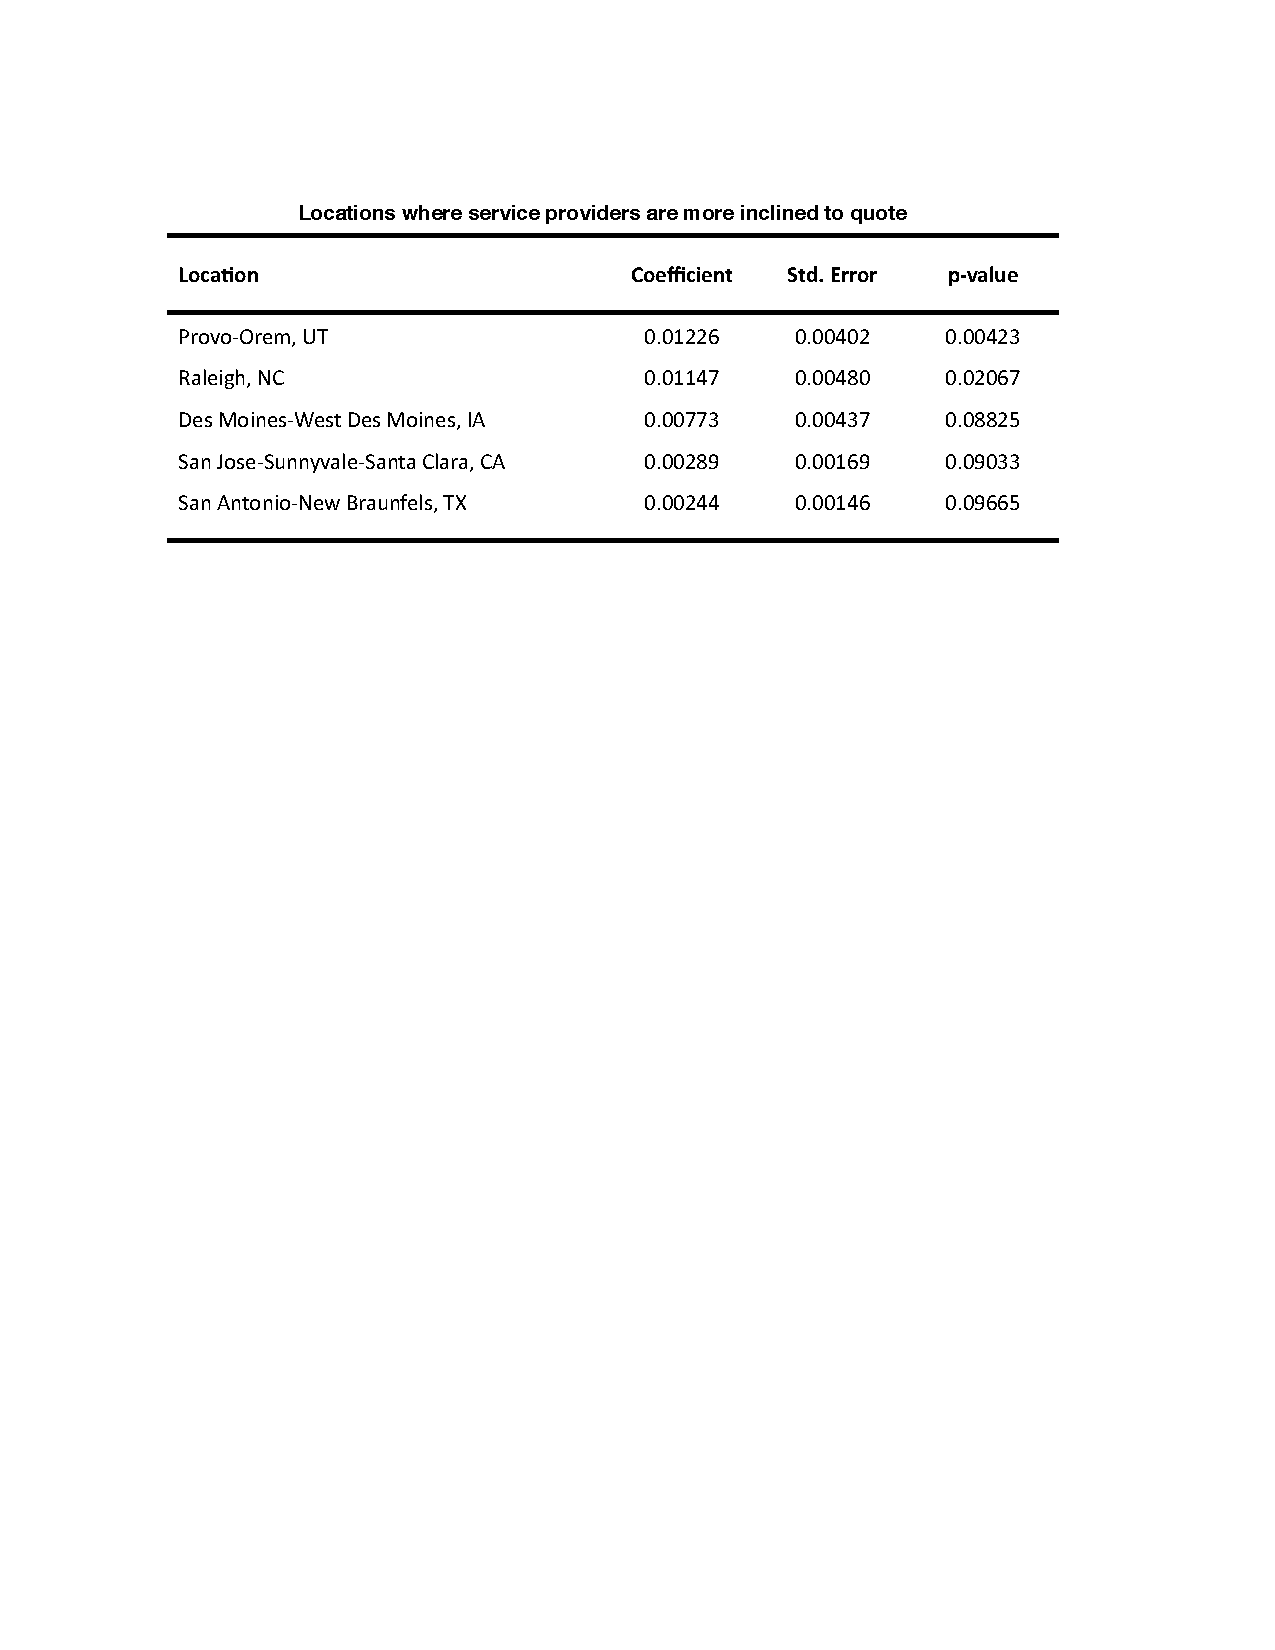
\includegraphics[scale=0.7]{coef_loc_more.pdf} }
	\end{figure}	
	\vspace*{-0 in}
\end{frame}

\begin{frame}{Behavior across Locations}{contd.}
	\vspace{-0.5 in}
	\begin{itemize}
		 \item{Locations with negative coefficients:}\newline  
	\end{itemize}
		\vspace{-0.5 in}
	\begin{figure}{}
		\vspace*{-0 in}
		\scalebox{1}
		{\hspace*{-0 in}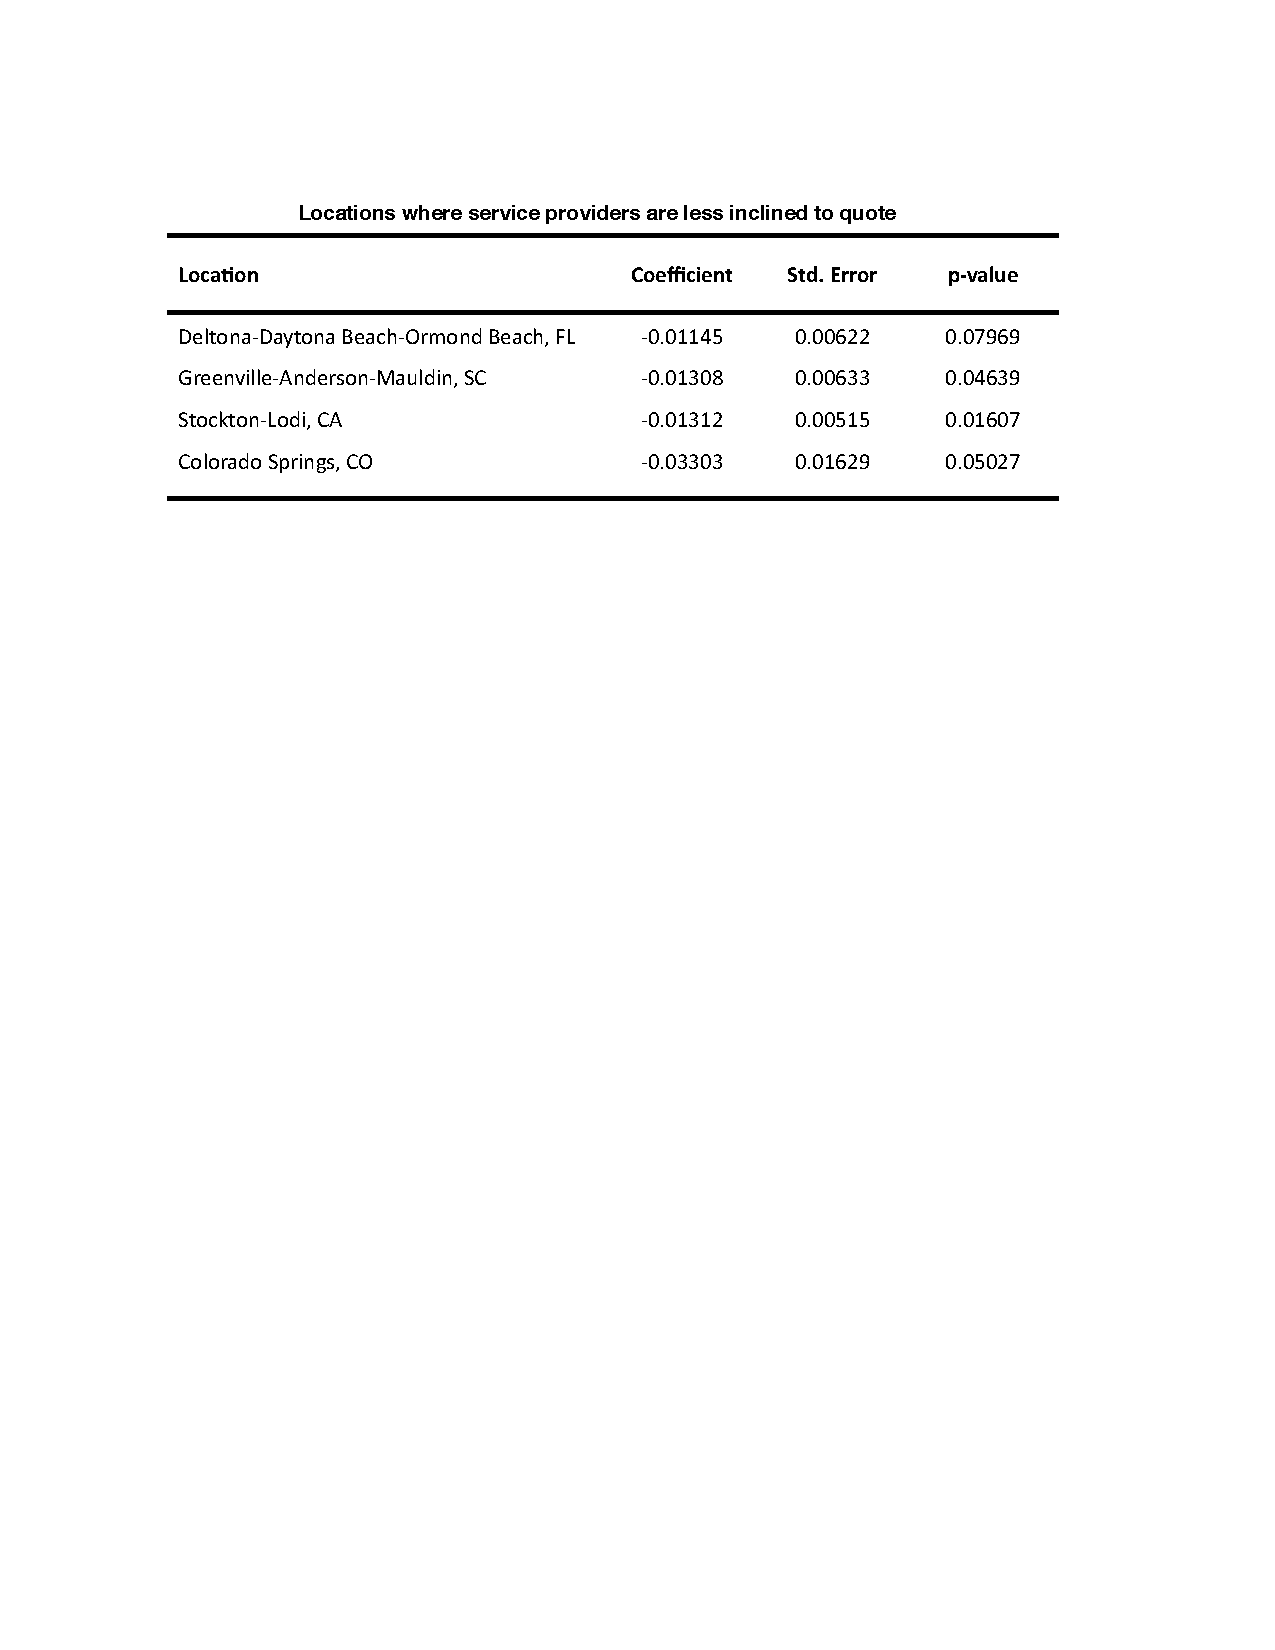
\includegraphics[scale=0.7]{coef_loc_less.pdf} }
	\end{figure}	
	\vspace*{-0 in}
\end{frame}

\begin{frame}{}{}
	\begin{center}
        		\Large{END}          
      \end{center}
\end{frame}

	
%		\item{Daily weighted growth in daily active users:} \newline
%		{$\LargerCdot$ percent growth in daily users divided by the day of growth.}\newline 
%		{$\LargerCdot$ assigns more weight to earlier add-ons.}\newline
%		\item{Average total admin:}\newline
%		{$\LargerCdot$ accounts for when were the admins. added.}\newline 
%		{$\LargerCdot$ admins. added later on would yield lower value.}\newline
%		\item{Average number of sessions per day:}\newline
%		{$\LargerCdot$ does not account for distinct admins.}\newline
%		\item{Average daily comments per session:} \newline
%		{$\LargerCdot$ daily comments divided by number of session, averaged over trial.}\newline
%		\item{Average duration per session per day:}\newline
%		{$\LargerCdot$ Time spent by admins.}\newline 



%
%\begin{frame}{Useful insights}{}
%	\begin{figure}{}
%		\vspace*{-0.1in}
%		\scalebox{0.85}
%		{\hspace*{-0.3 in}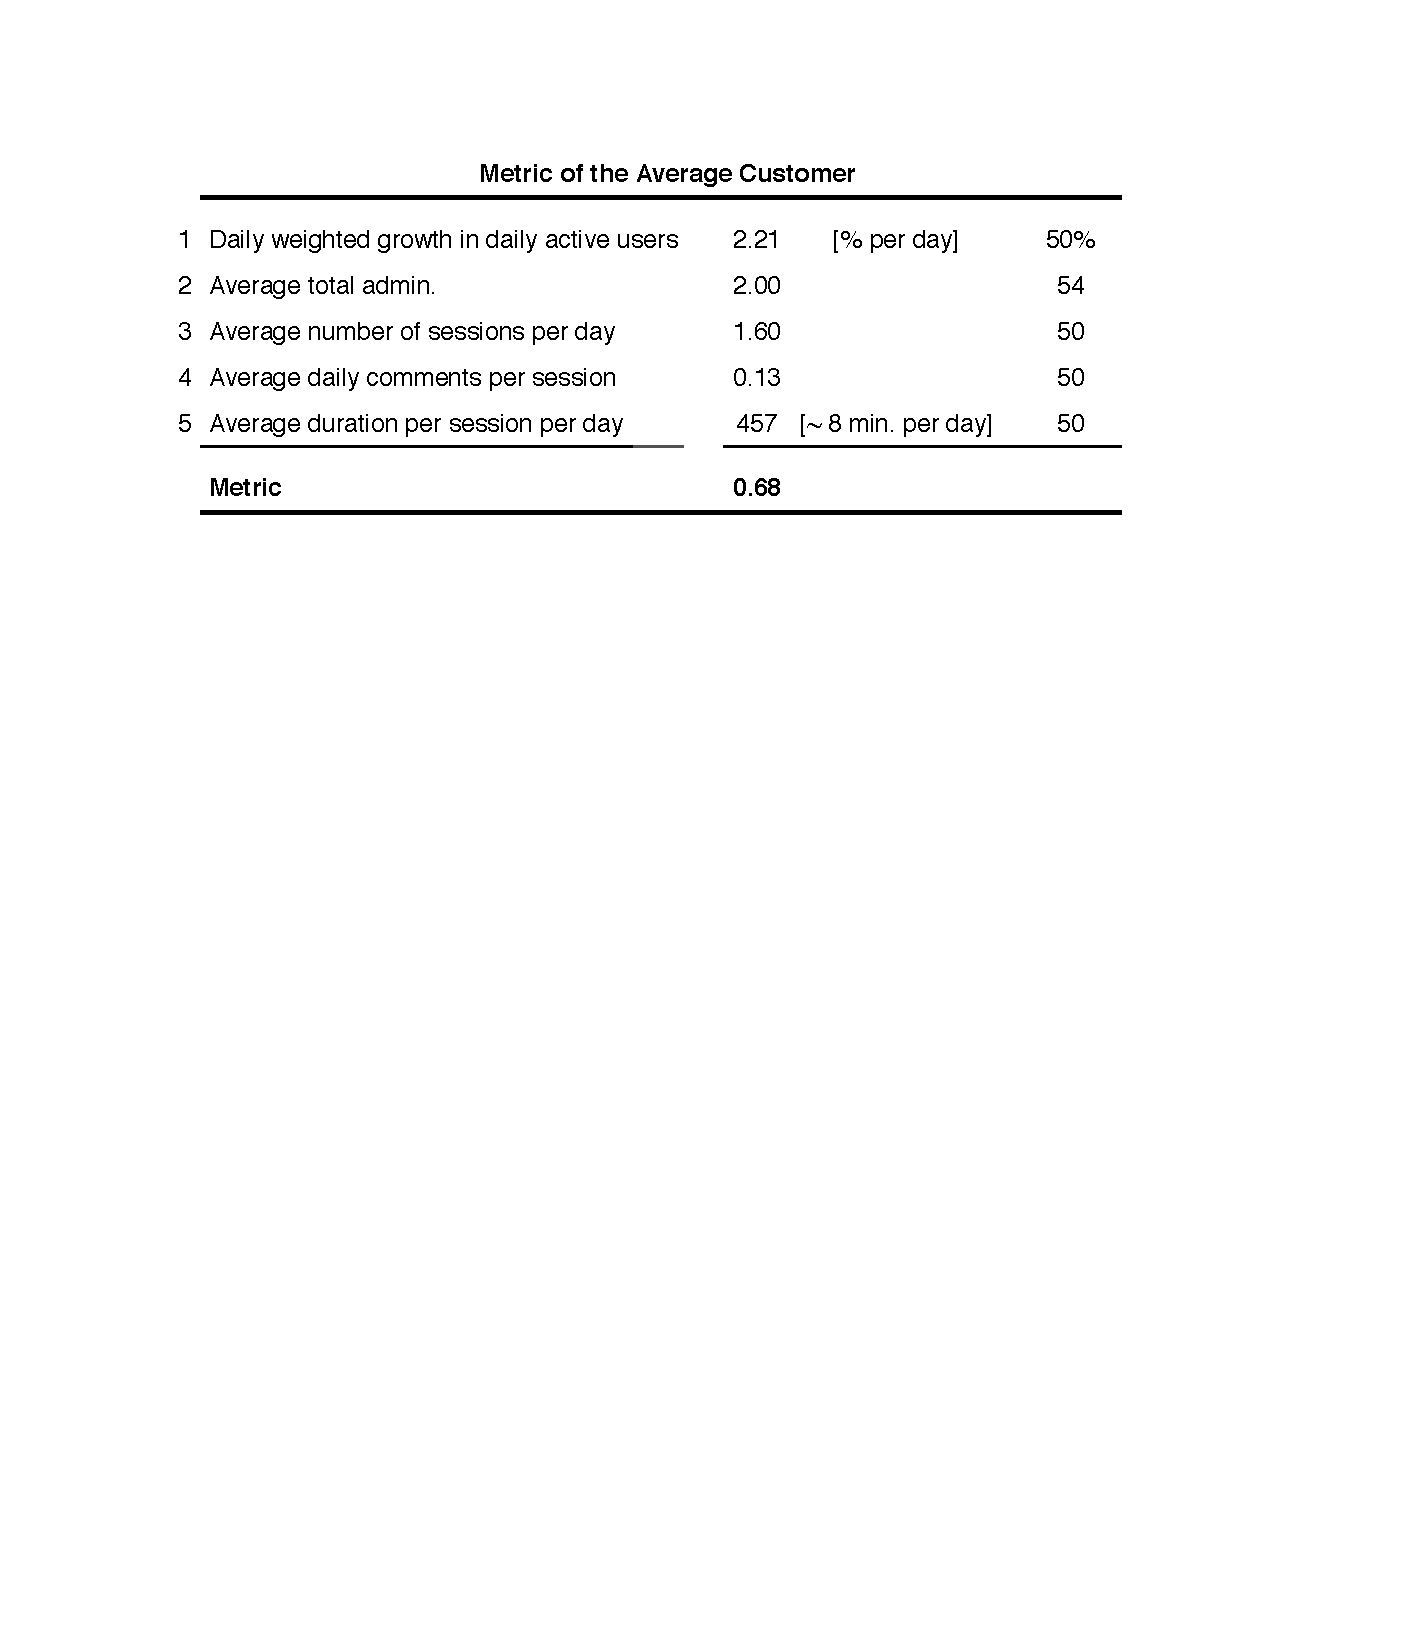
\includegraphics[scale=0.7]{results_summary_v3_fig2.pdf} }
%	\end{figure}
%	\vspace{-0.22in}
%	\begin{itemize}
%		\item{Trialling customers with Metric {\color{blue}above 0.65 convert to full-time customers.}}\newline
%%		\item{From all historical trialling customers: }\newline
%%		{$\LargerCdot$ 68\% generated a metric of above 0.65.}\newline
%		\item{From trialling customers that {\color{blue}converted}: }\newline
%		{$\LargerCdot$ 82\% generated a metric of above 0.65.}\newline
%		 \item{From trialling customers that \alert{did not convert}: }\newline
%		{$\LargerCdot$ 35\% generated a metric of above 0.65.}\newline
%	\end{itemize}
%\end{frame}
%
%\begin{frame}{Useful insights}{}
%	\begin{figure}{}
%		\vspace*{-0.1in}
%		\scalebox{0.85}
%		{\hspace*{-0.3 in}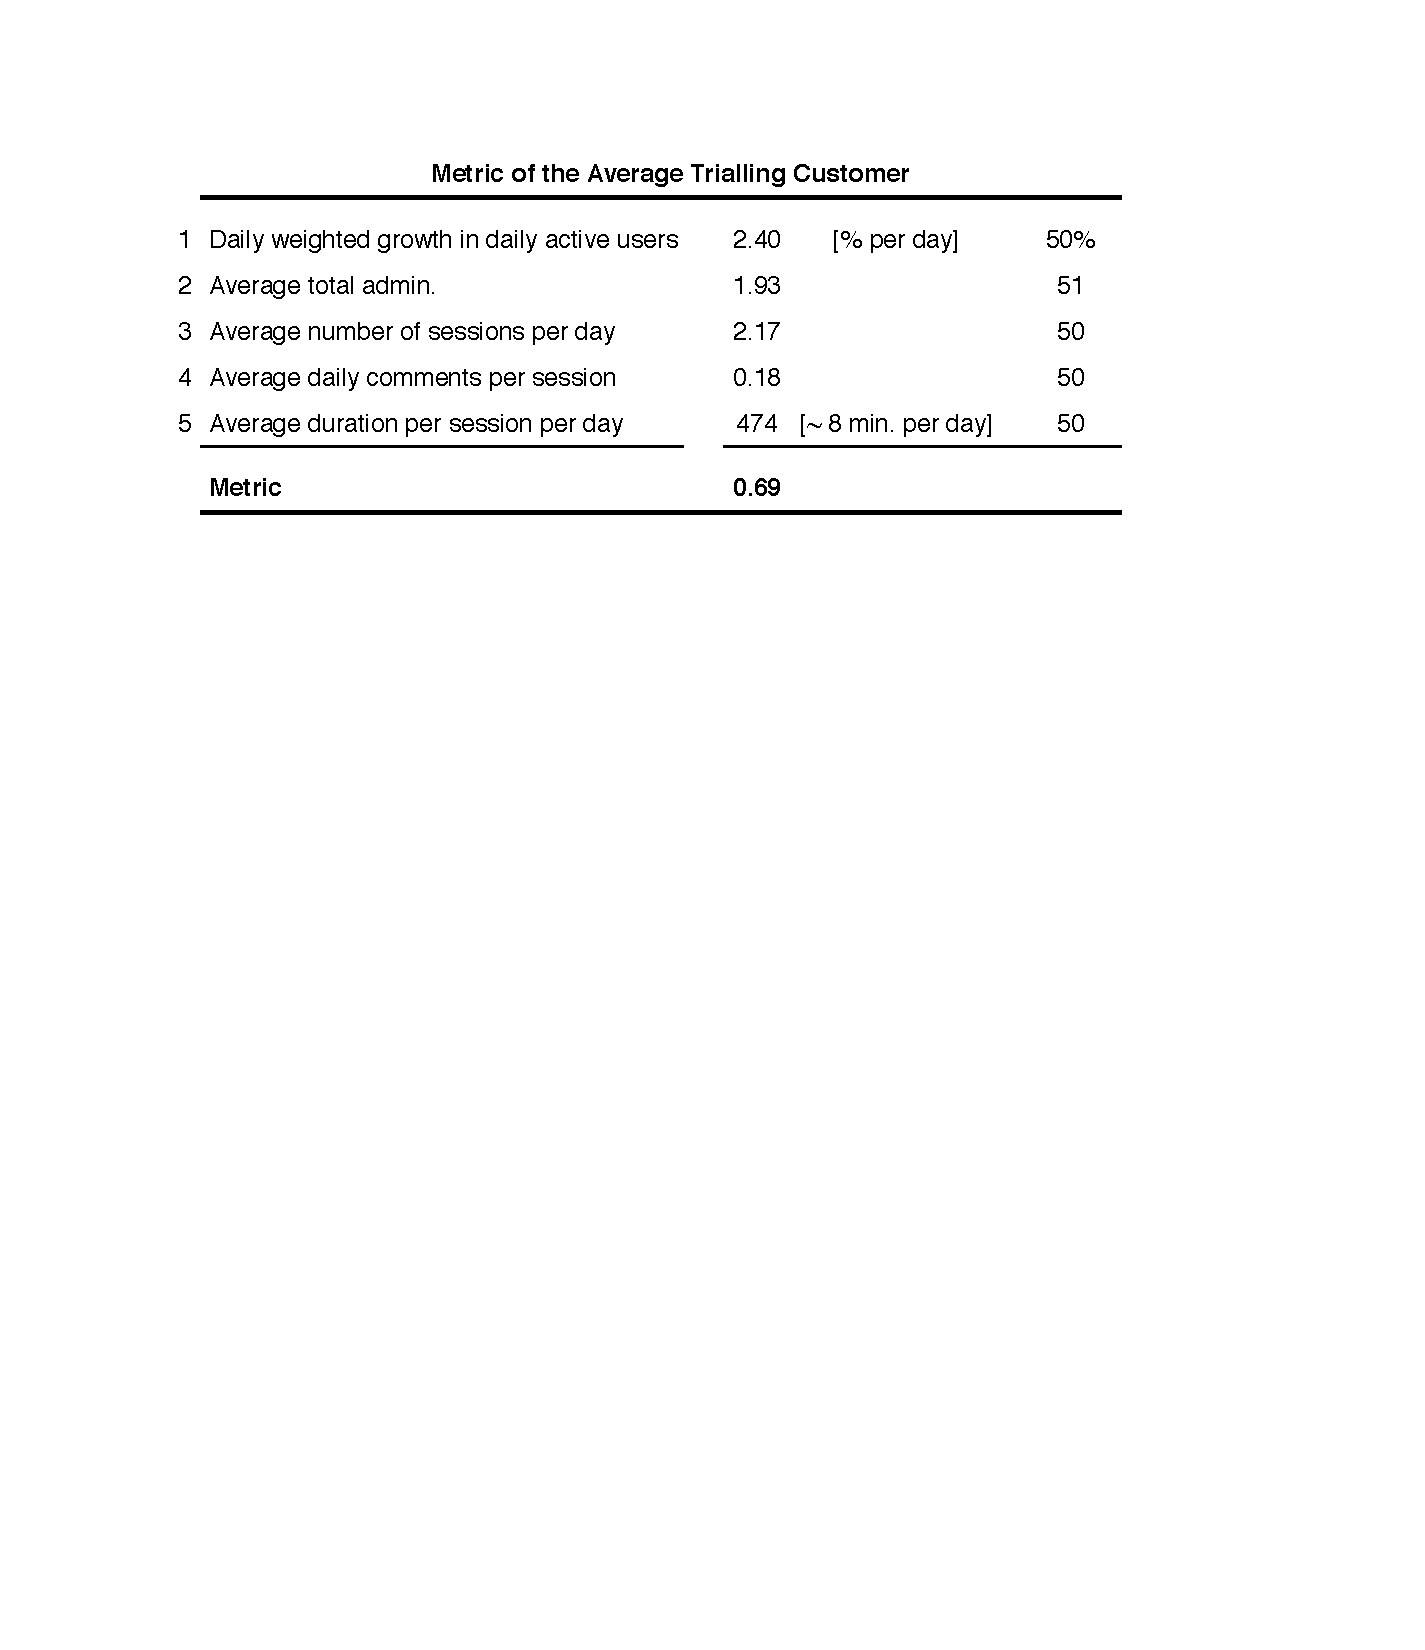
\includegraphics[scale=0.7]{results_summary_v3_fig3.pdf} }
%		{\hspace*{-0.12 in}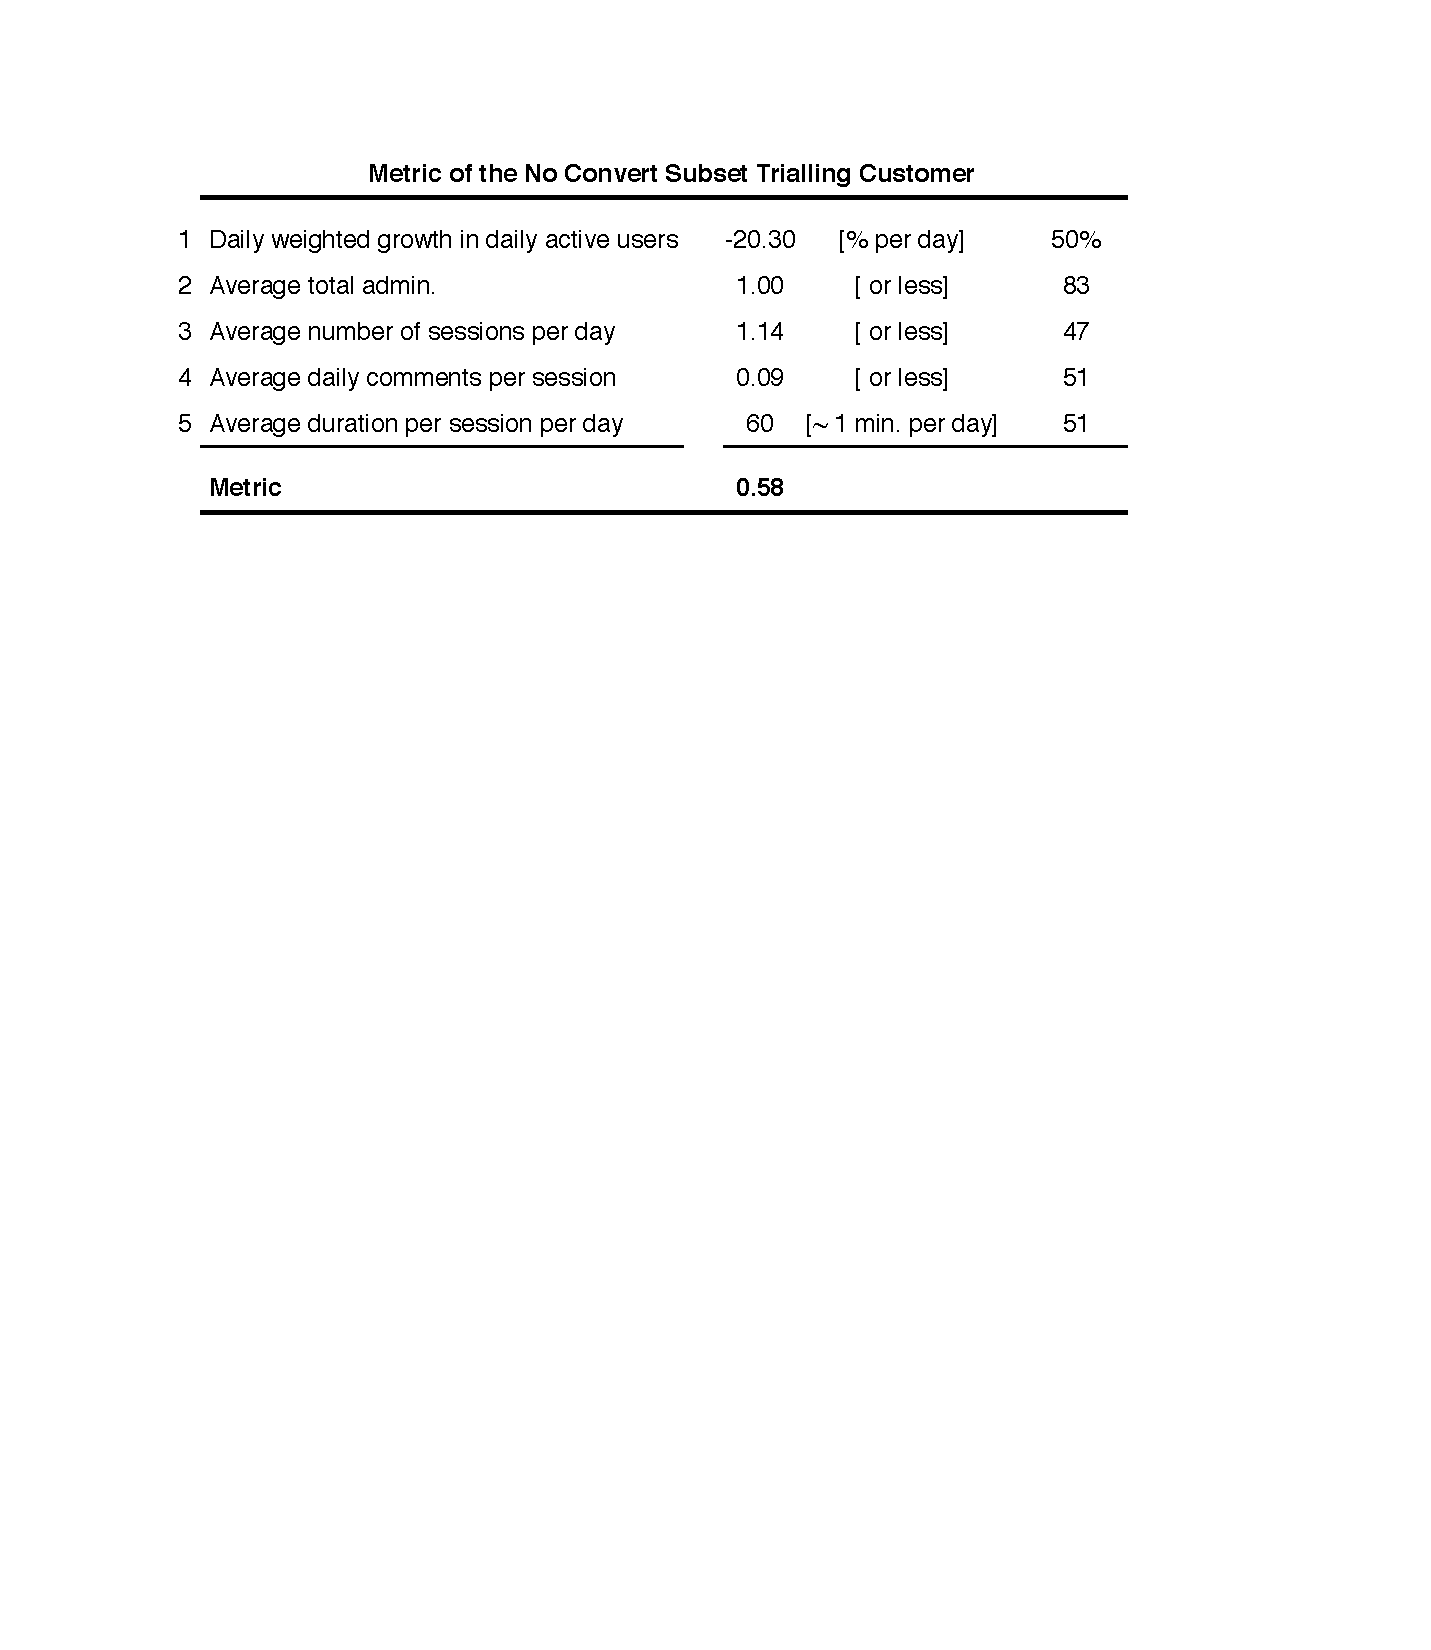
\includegraphics[scale=0.6]{results_summary_v3_fig4.pdf} }
%	\end{figure}
%\end{frame}
%
%\begin{frame}{Useful insights}{}
%%	\begin{figure}{}
%%		\vspace*{-0.1in}
%%		\scalebox{0.85}
%%		{\hspace*{-0.3 in}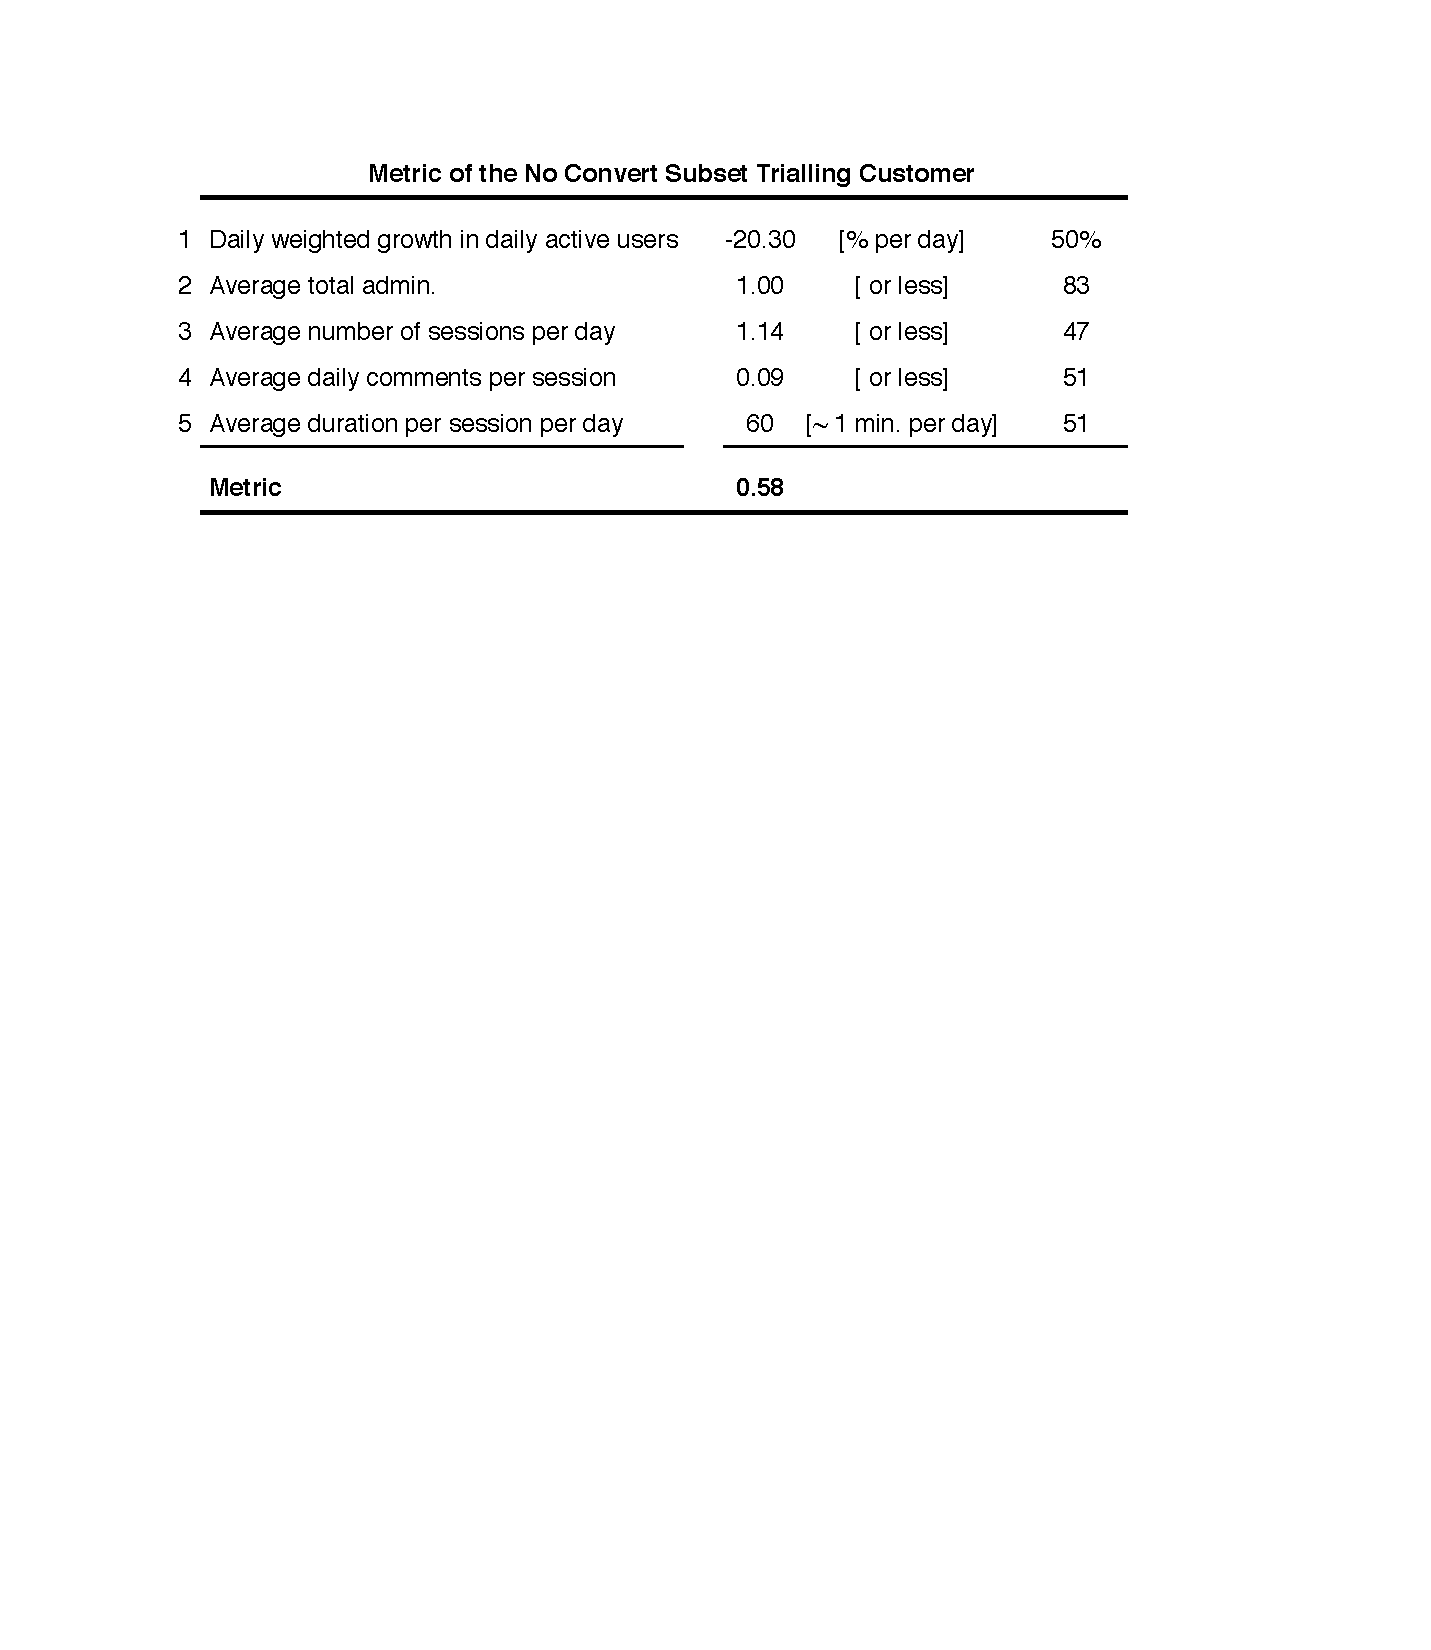
\includegraphics[scale=0.7]{results_summary_v3_fig4.pdf} }
%%	\end{figure}
%%	\vspace{-0.22in}
%	\begin{itemize}
%		\item{From current trialling customers {\color{blue} 72\% are expected to convert to full-time customers.}}\newline
%		\item{Measures to convert this subset of users: }\newline
%%		\item{From all historical trialling customers: }\newline
%		{$\LargerCdot$ Drive active daily users to increase daily weighted growth to $-10$\%.}\newline
%		{$\LargerCdot$ Get customer to add 1 more admin.}\newline
%		{$\LargerCdot$ Get the admin. to increase the number of sessions to 2 sessions per day.}\newline
%		{$\LargerCdot$ 	Get the users. to increase the number of comments by $10$\%.}\newline
%		{$\LargerCdot$ 	Get the admin. to spend $2$ minutes on the app per day.}\newline
%		\item{ This measure would convert {\color{blue} $82$\% of non-converting customers to full-time customers.}}
%	\end{itemize}
%\end{frame}


% All of the following is optional and typically not needed. 
%\appendix
%\section<presentation>*{\appendixname}
%\subsection<presentation>*{For Further Reading}
%
%\begin{frame}[allowframebreaks]
%  \frametitle<presentation>{For Further Reading}
%    
%  \begin{thebibliography}{10}
%    
%  \beamertemplatebookbibitems
%  % Start with overview books.
%
%  \bibitem{Author1990}
%    A.~Author.
%    \newblock {\em Handbook of Everything}.
%    \newblock Some Press, 1990.
% 
%    
%  \beamertemplatearticlebibitems
%  % Followed by interesting articles. Keep the list short. 
%
%  \bibitem{Someone2000}
%    S.~Someone.
%    \newblock On this and that.
%    \newblock {\em Journal of This and That}, 2(1):50--100,
%    2000.
%  \end{thebibliography}
%\end{frame}

\end{document}
